% Created by tikzDevice version 0.12.3.2 on 2022-04-24 21:04:01
% !TEX encoding = UTF-8 Unicode
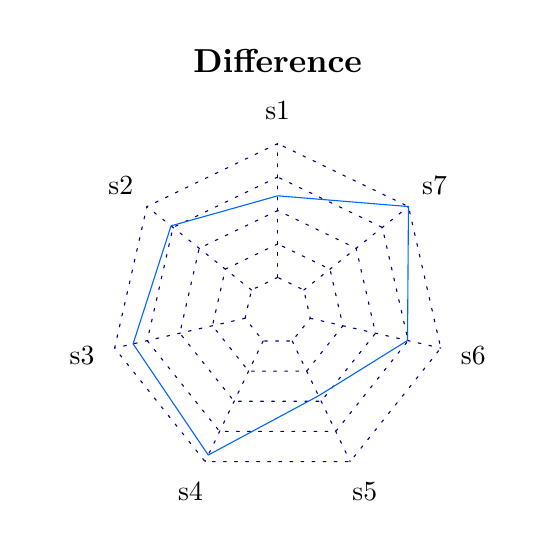
\begin{tikzpicture}[x=1pt,y=1pt]
\definecolor{fillColor}{RGB}{255,255,255}
\path[use as bounding box,fill=fillColor,fill opacity=0.00] (0,0) rectangle (180.67,180.67);
\begin{scope}
\path[clip] (  0.00,  0.00) rectangle (180.67,180.67);
\definecolor{drawColor}{RGB}{0,0,0}

\node[text=drawColor,anchor=base,inner sep=0pt, outer sep=0pt, scale=  1.20] at ( 90.34,164.53) {\bfseries Difference};
\end{scope}
\begin{scope}
\path[clip] (  0.00,  0.00) rectangle (180.67,156.67);
\definecolor{drawColor}{RGB}{0,0,128}

\path[draw=drawColor,line width= 0.4pt,dash pattern=on 1pt off 3pt ,line join=round,line cap=round] ( 90.34, 90.43) --
	( 80.89, 85.87) --
	( 78.55, 75.65) --
	( 85.09, 67.45) --
	( 95.58, 67.45) --
	(102.12, 75.65) --
	( 99.79, 85.87) --
	( 90.34, 90.43);

\path[draw=drawColor,line width= 0.4pt,dash pattern=on 1pt off 3pt ,line join=round,line cap=round] ( 90.34,102.52) --
	( 71.43, 93.41) --
	( 66.77, 72.96) --
	( 79.85, 56.55) --
	(100.83, 56.55) --
	(113.91, 72.96) --
	(109.24, 93.41) --
	( 90.34,102.52);

\path[draw=drawColor,line width= 0.4pt,dash pattern=on 1pt off 3pt ,line join=round,line cap=round] ( 90.34,114.60) --
	( 61.98,100.95) --
	( 54.98, 70.27) --
	( 74.60, 45.66) --
	(106.07, 45.66) --
	(125.70, 70.27) --
	(118.69,100.95) --
	( 90.34,114.60);

\path[draw=drawColor,line width= 0.4pt,dash pattern=on 1pt off 3pt ,line join=round,line cap=round] ( 90.34,126.69) --
	( 52.53,108.49) --
	( 43.19, 67.58) --
	( 69.36, 34.77) --
	(111.32, 34.77) --
	(137.48, 67.58) --
	(128.14,108.49) --
	( 90.34,126.69);

\path[draw=drawColor,line width= 0.4pt,dash pattern=on 1pt off 3pt ,line join=round,line cap=round] ( 90.34,138.78) --
	( 43.08,116.02) --
	( 31.41, 64.89) --
	( 64.11, 23.88) --
	(116.56, 23.88) --
	(149.27, 64.89) --
	(137.60,116.02) --
	( 90.34,138.78);

\path[draw=drawColor,line width= 0.4pt,dash pattern=on 1pt off 3pt ,line join=round,line cap=round] ( 90.34, 90.43) -- ( 90.34,138.78);

\path[draw=drawColor,line width= 0.4pt,dash pattern=on 1pt off 3pt ,line join=round,line cap=round] ( 80.89, 85.87) -- ( 43.08,116.02);

\path[draw=drawColor,line width= 0.4pt,dash pattern=on 1pt off 3pt ,line join=round,line cap=round] ( 78.55, 75.65) -- ( 31.41, 64.89);

\path[draw=drawColor,line width= 0.4pt,dash pattern=on 1pt off 3pt ,line join=round,line cap=round] ( 85.09, 67.45) -- ( 64.11, 23.88);

\path[draw=drawColor,line width= 0.4pt,dash pattern=on 1pt off 3pt ,line join=round,line cap=round] ( 95.58, 67.45) -- (116.56, 23.88);

\path[draw=drawColor,line width= 0.4pt,dash pattern=on 1pt off 3pt ,line join=round,line cap=round] (102.12, 75.65) -- (149.27, 64.89);

\path[draw=drawColor,line width= 0.4pt,dash pattern=on 1pt off 3pt ,line join=round,line cap=round] ( 99.79, 85.87) -- (137.60,116.02);
\definecolor{drawColor}{RGB}{0,0,0}

\node[text=drawColor,anchor=base,inner sep=0pt, outer sep=0pt, scale=  1.00] at ( 90.34,147.66) {s1};

\node[text=drawColor,anchor=base,inner sep=0pt, outer sep=0pt, scale=  1.00] at ( 33.63,120.35) {s2};

\node[text=drawColor,anchor=base,inner sep=0pt, outer sep=0pt, scale=  1.00] at ( 19.62, 58.99) {s3};

\node[text=drawColor,anchor=base,inner sep=0pt, outer sep=0pt, scale=  1.00] at ( 58.87,  9.78) {s4};

\node[text=drawColor,anchor=base,inner sep=0pt, outer sep=0pt, scale=  1.00] at (121.81,  9.78) {s5};

\node[text=drawColor,anchor=base,inner sep=0pt, outer sep=0pt, scale=  1.00] at (161.05, 58.99) {s6};

\node[text=drawColor,anchor=base,inner sep=0pt, outer sep=0pt, scale=  1.00] at (147.05,120.35) {s7};
\definecolor{drawColor}{RGB}{0,102,255}

\path[draw=drawColor,line width= 0.4pt,line join=round,line cap=round] ( 90.34,119.91) --
	( 51.81,109.06) --
	( 38.09, 66.41) --
	( 65.25, 26.24) --
	(105.12, 47.65) --
	(137.25, 67.63) --
	(137.60,116.02) --
	( 90.34,119.91);
\end{scope}
\end{tikzpicture}
